{
\setlength{\parindent}{2em}
\chapter{State of the Art}\label{cha:state-of-the-art}
Saving the state of a running application to a file has been a very well-known challenge in the world of computer science, one that has its roots back to when the computers became powerful enough to run complicated programs. With the rise of local networks and the Ethernet protocol in the 1970s, an increasing amount of processing units could be linked together through a local network in order to improve the execution speed of difficult computation \cite{book:andrews}. This gave rise to the field of distributed computing, where scalability, parallelization of algorithms and efficient inter-node communication are among the very active topics of research.

Of course, the more complicated a system is, the more failure-prone it becomes. This is why it's imperative for designers of parallel algorithms to be careful when programming their application. It has to be made in such a way that it stays tolerant to eventual faults in the computing nodes of the network. For instance, one can think of the algorithms involved in numerical weather prediction software, that theoretically never finish as long as updated data is fed into the system. It is important for the forecasting industry not to loose any of the results that were previously solved if an unfortunate event occurs. \textit{Fault-tolerant computing} is the research field that finds solutions to this problem in multiple ways. In the context of distributed computing, one of the ways to mitigate the problem is to use a checkpoint and restart mechanism.

This technique allows the program to save itself while it's running, and to restart at a previous checkpoint. A "save" can take many forms, and its content is ultimately decided by the developers of the program. Before a final design is produced, some questions need to be answered:
\begin{enumerate}
	\item \textbf{What needs to be saved?} There needs to be a clear understanding of the program and how it works. Is saving only the intermediate result of a computation considered a sufficient condition to be able to restore the program back to where it was? Is saving the entire state of the operating system required? Of the entire computer? 
	\item \textbf{In which format should the data be saved?} This can be binary data, numerical data, text, etc. This is again highly dependent on the application. A suitable file format has to be used depending on the data to store.
	\item \textbf{How is the data saved?} How can a checkpoint take form? This depends on the content. Most of the time, this will be a file written to non-volatile memory. Again, the file format has a role to play.
	\item \textbf{How often is saving necessary?} A checkpoint can take a lot of space, and that amount usually grows linearly with the number of execution threads. In huge systems, this is not a trivial question. In addition, not only does a checkpoint take up hard disk space, it also induces an overhead in the execution of the program. Depending on the desired granularity, saving the relevant data can take a significant amount of time. This is represented by $O_F$ in \autoref{fig:chkpt-scheme}. This factor is important, especially in big distributed systems where computing time is expensive. As an example, the Titan supercomputer in the United States racks up \$9 million USD in electricity bills yearly \cite{online:henn}.
	\item \textbf{How long does it take to restart?} Saving at checkpoints takes time, but so does recovery. \autoref{fig:chkpt-scheme} shows this with $R_F$. Another point to consider is how often the system needs to restart back. In the end, restarting to a past state must be as straightforward as possible.
\end{enumerate}
\begin{figure}[H]
	\centering
	\includesvg[width=0.9\linewidth]{svg/chkpt-copy}
	\caption{Checkpoint/restart as a stochastic renewal reward process.\cite{misc:chkpt-scheme}}
	\label{fig:chkpt-scheme}
\end{figure}

\subsection*{Checkpointing Schemes}
There are different checkpointing schemes that are adapted to different needs. On one hand, it is possible to checkpoint the application at predetermined intervals $\Delta t$ (i.e every minute). This is useful when applicable, because it puts an upper bound on the amount of data/time loss in a worst case scenario. However, this mitigation method is not always possible for every type of computation. 

The second approach is to do it sporadically. This can be used when it's impossible to predict the amount of time required for a given computation. Unfortunately, it also means that the user doesn't know exactly when checkpoints will occur nor can she/he upper-bound the maximum amount of data/time loss.

\subsection*{Applicability to BBPSim}
Why exactly can these concepts be useful in the case of a simulator like BBPSim? The checkpoint and restart technique is not only applicable to the distributed computing, it can be adapted to fit the needs of multiple kinds of programs. At the very least, some of the concepts can serve as inspiration to design a save \& restore feature. In the following sections, some existing \textit{snapshotting} solutions in released software will be investigated. Using available source code and documentation, it will be possible to see that a checkpoint/restart feature can be implemented at different levels. In the end, the analysis will extract a set of working ideas as inspiration for the save \& restore in BBPSim.

%---state of the art analysis
\section{VirtualBox}\label{sec:virtualbox}
This open-source software project backed by Oracle is well-known in the virtualization industry. It is a hypervisor, a type of program defined by Red Hat as a
\begin{shadedquotation}
	[...] software that creates and runs [one or more] \gls{VM}. A hypervisor, sometimes called a \gls{VMM}, isolates the hypervisor operating system and resources from the virtual machines and enables the creation and management of those VMs.\cite{online:redhat}
\end{shadedquotation}
Indeed, VirtualBox acts as a mediator between a guest OS (the \textit{virtualized} OS) and a host OS. It is labeled as a Type-2 hypervisor, meaning that it is actually a software layer that separates both operating system, as \autoref{fig:layerhyper} shows. VirtualBox is in charge of exposing computer utilities to the guest operating system, like CPU time, RAM allocation, driver and graphics card access, etc. Like most of its counterparts, the hypervisor also offers to the user the possibility of manually (\textbf{sporadically}) \textit{snapshotting} a virtual machine's current state in order to allow a future restore to exactly this state : the state of the drivers, running process scheduling information, even the graphical interface. The feature outputs a sizable file as a result.

\begin{wrapfigure}{r}{0.45\textwidth}
	\centering \scriptsize
	\vspace{-12pt}
	\includesvg[width=0.37\textwidth]{svg/hypervisor}
	\caption{Abstraction layers for a type-2 hypervisor.}
	\label{fig:layerhyper}
	\vspace{-24pt}
\end{wrapfigure}
This application being open-source, it's possible to dive deeper and investigate the code ourselves \cite{online:vboxcode}. We are mostly interested here at how VirtualBox handles the saving of guest OS processes and memory, since BBPSim doesn't have a graphical interface nor uses the typical PC peripherals like USB or the audio output.

From the root of the code repository, we can find the \pathmono{src/VBox/Main/src-server/SnapshotImpl.cpp} file that contains interesting \Cpp classes and routines. We can see that \cppsym{SessionMachine::i_takeSnapshotHandler} is the method responsible for the snapshot feature. The feature does many things, but four snapshot aspects stand out by how they approached their design to make the saving problem possible.

\subsection*{Snapshotting process}

VirtualBox needs an efficient strategy to save the general state of the virtual machine. Precisely, it is VBox's Saved State Manager's (SSM) responsibility to implement the facilities for saving and restoring a VM state in a structural manner.

During initialization of a given virtual machine (i.e right before the guest OS starts its boot sequence), the SSM registers the different virtual components that are available to the virtualized operating system. When time comes for the user to hit the \inlinegraphics{art/take-snap.png} button while the VM is running, the Saved State Manager goes through its list of registered components. The components then save their internal state themselves using the API the SSM provides, and the SSM takes care of encoding the data. As a result, what is called a "stream" in the project is produced from the agglomeration of the saved data. This is a powerful way of dealing with this problem and has many advantages :
\begin{enumerate}
	\item Encapsulation is kept since each component takes care of saving itself. This is good for software maintenance.
	\item Adding a new component to include in a save only requires it to register itself at initialization. The SSM doesn't need to be aware of the capabilities said component provides.
	\item The time to save a machine's state grows linearly with the number of components, since they are completely decoupled from each other.
\end{enumerate}

\hfill\textit{Relevant file }: \pathmono{src/VBox/VMM/VMMR3/SSM.cpp}.

\subsection*{Non-volatile Memory Snapshot}

From a hard disk point of view, the hypervisor takes an interesting \textit{diff}-based approach. This means that from the time a snapshot is created, VirtualBox associates it with a list $L$ of changes in which all $n$  subsequent hard disk write operations $w$ are added. When the user wants to comeback to a certain snapshot taken at time $t_0$, the \gls{VMM} then takes the current state of the disk ($\text{HDD}_{tn}$) and traverses $L$ in the reverse order while applying the inverse operation.
\[
\text{HDD}_{t0} = \text{HDD}_{tn} + \sum_{i=n}^{0}w_i^{-1}
\]
This effectively undos all previous operations. Using this technique means that \ul{VirtualBox snapshots are dynamic objects} that grow linearly with the subsequent usage of their affiliated VM.

\hfill\textit{Relevant file }: \pathmono{src/VBox/VMM/VMMR3/SSM.cpp}.

\subsection*{CPU State Snapshot}

As for the saving of the CPU state itself, the CPU Monitor (CM) is responsible for keeping track of all the CPU and \gls{FPU} registers while the virtual machine is running. In practice, the exact identity of all those registers depends on the architecture of the host hardware (assumed to be x86) and the host OS. For instance, a 32-bit OS would be using the "extended" (\textit{E}-prefixed) registers, like in \autoref{fig:x86-regs}. 
\begin{figure}[H]
	\centering
	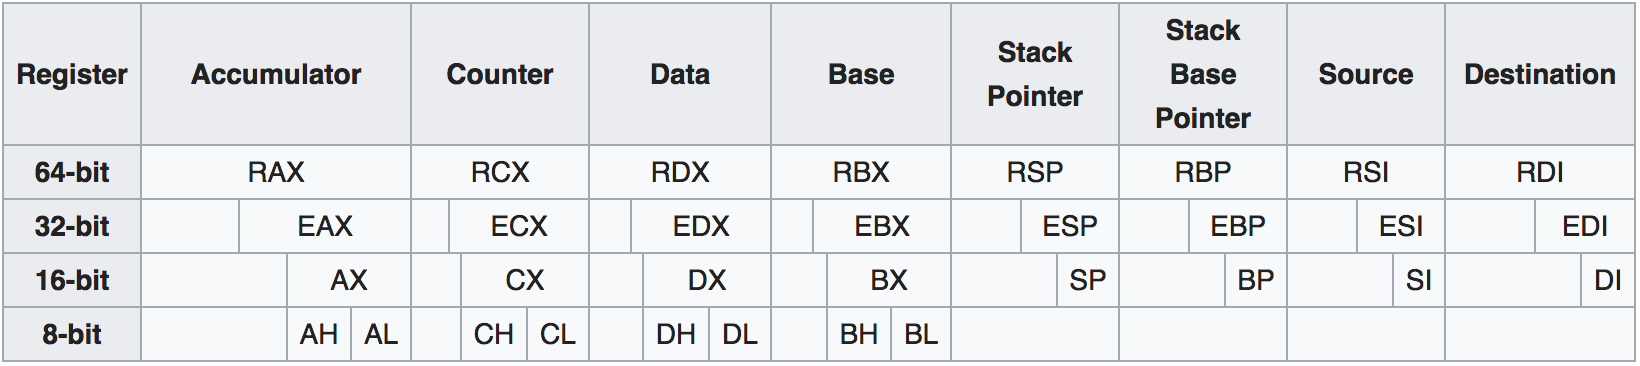
\includegraphics[width=.85\linewidth,keepaspectratio]{art/x86-regs.png}
	\caption{Usage of basic registers ordered by word size of the operating system on the x86 architecture.}
	\label{fig:x86-regs}
\end{figure}
The state (i.e value) of all the relevant CPU registers at a time $t$ is called a \textbf{context}. In VirtualBox, the CM keeps local copies of three of these contexts : a guest OS context, a special hypervisor context for the VMM and a raw context (a normal host OS context). When making a snapshot of the VM, the CPU Monitor actually saves the first two in order to subsequently put back the CPU exactly like it was at time $t$. Beside the saving aspect, holding three different contexts also allows VirtualBox to quickly switch between the guest and host "worlds" without the user noticing. This is very much necessary, because the whole point of the hypervisor is to make two different operating system coexist at the same time.

\hfill\textit{Relevant file }: \pathmono{src/VBox/VMM/VMMR3/CM.cpp}.

\subsection*{RAM Snapshot}

Another extremely important aspect of the state save is the dynamic memory aspect. How can VirtualBox completely separate the guest OS from the host without the guest noticing? This is done through the Page Manager (PM), a manager also taken into account by the Saved State Manager at snapshot time. 

\begin{wrapfigure}{l}{0.45\textwidth}
	\centering \scriptsize
	\vspace{-12pt}
	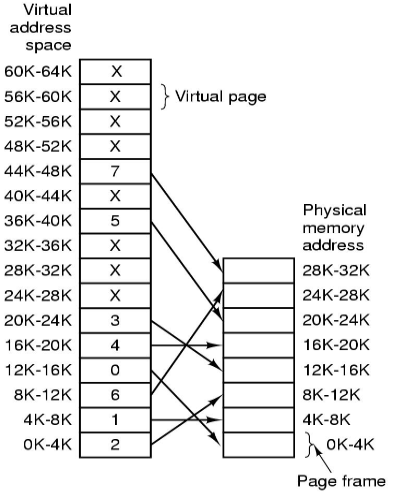
\includegraphics[width=0.40\textwidth,keepaspectratio]{art/mem-paging.png}
	\caption{Linux Mapping of Pages to Page Frames \cite{misc:mem-paging}}
	\label{fig:mem-paging}
	\vspace{-12pt}
\end{wrapfigure}
To better understand the Page Manager's job, we can look at a very similar concept : the memory paging technique used by the Linux operating system. As shown in \autoref{fig:mem-paging}, the way Linux abstracts the hardware from a running program is by offering said program an entire virtual address space as a sandbox. 

This virtual space is divided into fixed-length memory blocks (usually 4kB) called virtual pages that have a one-to-one correspondence to a random block of the same size in physical memory (page frame). Linux abstracts that correspondence with the help of a \gls{MMU} implemented in hardware, which translates virtual addresses into physical ones.

In the same way that Linux controls VirtualBox's physical memory accesses, the Page Manager controls the guest OS memory accesses. It enables the management of pages of memory allocated by the guest and adds one more level of memory indirection. For example, a program running on the guest OS will be executing operations on guest memory, but VirtualBox actually redirects them to operate directly on the physical address space offered by the host OS. This can be done with the help of two powerful concepts:
\begin{enumerate}
	\item \textbf{Binary translation}. This allows a software-assisted hypervisor like VirtualBox to "trap and virtualize the execution of sensitive, non-virtualizable instructions sets"\cite{online:virtualization}, like memory operations.
	\item \textbf{\gls{SLAT}}. Commonly known as \textbf{nested paging}, it allows a guest operating system to directly access the host's physical memory and thus removing a lot of overhead on memory operations.
\end{enumerate} 

Because the \gls{VMM} can hook to these memory operations in the guest OS, this makes the Page Manager aware of the page frames that belong to the guest OS. As a result, when a snapshot event occurs, the PM goes through its list of guest pages that were in use at that time and saves them. At restore time, this data is copied back someplace else in physical memory, and the translation table is updated accordingly.
 
\hfill\textit{Relevant file }: \pathmono{src/VBox/VMM/VMMR3/PGM.cpp}.
\section{Checkpoint and Restore in User Space (CRIU)}\label{sec:criu}
As mentioned previously, the problem of checkpointing a computer program can be solved at multiple levels depending on the needs. The approach that was taken by VirtualBox is very powerful, but it has major drawbacks:
\begin{enumerate}
	\item \textbf{Overhead processing}. The fact that an entire system gets simulated implies that virtualizing an operating system with a type-2 hypervisor like VirtualBox is basically an overhead cost on executing the program. 
	\item \textbf{Granularity}. It checkpoints the whole computer's state instead of one program. This is often too much granularity and can result in very large snapshot files. In the case of \gls{BBPSim}, this would be quite excessive.
	\item \textbf{Dependence on an hypervisor}. If the execution of the program had to happen inside a virtualized operating system, a simulation of the \gls{BBP} would have to rely on the use of an hypervisor. This not desirable, especially from the client's perspective.
\end{enumerate}

However, some other techniques can circumvent these limitations by using a differing degree of checkpointing transparency, that is, at which abstraction layer the checkpoint takes place. Walters and Chaudhary define those layers as follows: 
\begin{shadedquotation}
\begin{enumerate}
	\item Hardware-level, additional hardware is incorporated into the processor to
save state.
	\item Kernel-level, the operating system is primarily responsible for checkpointing
running programs.
	\item User-level, a checkpointing library is linked into a program that will be responsible for checkpointing the program independent of the programmer.
	\item Application-level, the checkpointing code is inserted directly into the application by a programmer/preprocessor.
\end{enumerate}
\cite{paper:app-level-chkpt}
\end{shadedquotation}

\gls{CRIU} is one those attempts at creating a user-friendly method for checkpointing a Linux program. It is an open-source program \cite{online:criucode} implemented at the user-level, meaning that a piece of software has to run in parallel to the program itself. CRIU has the benefit of not needing to run privileged instructions like a kernel-level checkpointing program would do. However, it still needs a bit of cooperation from the Linux kernel for certain operations.

\subsection*{Overview}
\gls{CRIU}'s solution is completely different from the one seen in \autoref{sec:virtualbox}, where saving happens for every program running in the guest OS. It bases itself on the fact that it is possible for a user-linked checkpointer library to:
\begin{itemize}
	\item Hook on a checkpointee's system calls during its execution.
	\item Alter the relevant system calls before they get sent to the OS.
	\item Keep track of which resources the checkpointee possesses or operates on with the help of the kernel.
\end{itemize}
The action of saving a program is managed by a remote procedure call (RPC) daemon, which runs in background and executes a "dump" (checkpoint) of a given program. 
\begin{figure}[htbp]
	\centering \small
	\includesvg[width=0.75\textwidth]{svg/criu}
	\caption{Location of the different layers of the CRIU saving ecosystem.}
	\label{fig:layercriu}
\end{figure}

There are several different ways to use \gls{CRIU}. An application-centric use case is shown in \autoref{fig:layercriu}. First, to access the required utilities for checkpointing, the application code needs to have access to the library's API at compile-time. At run-time, the \pathmono{libcriu.so} is dynamically linked to the code and CRIU starts to monitor the application's resources by intercepting low-level activity (usually Linux system calls). Then, it alters the calls to give the access to data normally application-private. This management layer is the key to monitoring the actions of the checkpointee and the focal point of the CRIU environment.

Sending a "dump" command from the application's code may be done via C API calls to CRIU's dynamic library:
\begin{minted}{c}
int criu_dump(void);
\end{minted}
This function is called programatically by the running application to checkpoint itself. It is an abstraction for remote procedure calls that are sent to the CRIU ecosystem. Once those commands are initiated, the \gls{CRIU} RPC daemon outputs a series of files containing sufficient information to restart back the application at that point. Data concerning the execution state of child threads and processes, as well as the different virtual address spaces' memory pages are part of the content of the output files.

At restore time, the checkpointee can call another C API function to do so: 
\begin{minted}{c}
int criu_restore(void);
\end{minted}
This fully restores the old application's state: virtual address space, registers, thread and process IDs, file descriptors, signals. Basically everything not related to sockets or serial ports is put back the way it was.

Beside that, an external user can also control the program from outside, using shell commands that connect directly to the RPC daemon:
\begin{minted}{bash}
criu dump -D <outdir> -t <pid>
criu restore -D <outdir>
\end{minted}

\subsection*{Non-volatile Memory Snapshot}
Because Checkpoint and Restore in User Space doesn't operate as an entire layer directly under the program to checkpoint, and because the changes in the Linux file system are persistent from one program run to another, there is no need for CRIU to save all the operations made on disk like VirtualBox. 

There is however an edge case when the program is saved while it possesses a handle to an opened file. In Linux, because every file operation is done through system calls, the interception layer is able to catch the relevant file's path. At restore, CRIU reopens the same files or, if the files aren't there anymore, invalidates the handle variables (in C: \mintinline[]{c}|FILE* fd;|). 

\hfill\textit{Relevant file }: \pathmono{criu/fdstore.c}.

\subsection*{CPU State and Execution Snapshot}
As stated previously, Checkpoint and Restore in User Space is able to take a snapshot of an entire tree of process IDs (pid). Inside the kernel, these pids represent an identifier given to all the threads of execution currently active inside Linux. Since each thread is composed of its own context with its own registers set values, CRIU must save the register set of all the threads that own an identifier related to the checkpointed program.

Once again, the process is made much more easier because of CRIU's interception layer. Since it is registered as a "tracer" in relation to the checkpointee, it is able to send commands to the Linux kernel to get the registers of all the threads that should be saved. This is done using the \mintinline[]{c}|ptrace()| process-to-process interface.
\begin{shadedquotation}
The ptrace() system call provides a means by which one process (the "tracer") may observe and control the execution of another process (the "tracee"), and examine and change the tracee's memory and registers.  It is primarily used to implement breakpoint debugging and system call tracing.
\cite{on:ptrace}
\end{shadedquotation}
Since CRIU is registered as a tracer, it is possible for it to gather the registers of the application's threads simply by referring directly to Linux. This can be done simply with:
\begin{minted}{c}
ptrace(PTRACE_GETREGSET, pid, NT_PRSTATUS, &regs);
\end{minted}
The registers CRIU then gets depends on the architecture of the computer. Nevertheless, this call requires the traced thread to be stopped in order to succeed.

\hfill\textit{Relevant file (x86-64)}: \pathmono{criu/compel/arch/aarch64/src/lib/infect.c}.

\subsection*{RAM Snapshot}
From CRIU's perspective, memory inside the \gls{VMA} of the traced process is handed out by the OS in pages (about 4kB). In fact, the complete set of virtual pages that the tracee possesses is required for the checkpointing program to restore it in a stable condition. Incidentally, the Linux operating system provides a very useful API in that regard:
\begin{minted}{bash}
pmap -x <pid>
\end{minted}
The command lists the address and size of the different allocated sections inside the tracee's \gls{VMA} range. In addition, the utility gives the "dirtyness"  (whether the section has once been written to), the permissions and even the mapping (if the section is code, stack, shared object, etc.) each section is associated with. The usage of \mintinline[]{bash}|pmap| doesn't require elevated privileges. However, since a read-write access to the content of the memory pages from other applications is forbidden for security reasons, CRIU is required to "be present" inside the checkpointee's virtual memory address range. This is the reason why \pathmono{libcriu.so} has to be linked in the compilation phase and loaded at runtime. 

When executing a "dump" operation, CRIU fetches the list of memory pages part of the checkpointee's VMA range and saves them one-by-one. 

\hfill\textit{Relevant file }: \pathmono{criu/mem.c}.
\section{Cornell Checkpoint Compiler (C\textsuperscript{3})}\label{sec:c3}
In the previous sections, various approaches for checkpointing an application from an outside entity were explained. In particular, it was shown in \autoref{sec:virtualbox} that VirtualBox interprets the computer instructions that run on the guest operating system, and transforms them to host-runnable instructions via binary translation, keeping a reference to the resources allocated for the guest. 
Then, \autoref{sec:criu} showed how an outside checkpointing program could layer itself between the checkpointee and the OS, in order to register their important interactions related to resources access and allocation. 

From the checkpointee's point of view, both of these techniques never really have a direct effect. They divert and reinterpret the instructions, resource usage, etc., but never influence the internal algorithms functionally. The program always yields the same result.

Although these methods of checkpointing have big transparency benefits by not modifying the program, in the context of big distributed systems, where there can be many millions of CPU cores, their caveats are amplified:
\begin{itemize}
	\item VirtualBox's snapshot size is a huge bottleneck. For each computer, there would be several gigabytes of RAM to save, which quickly becomes unpractical. In addition, for high performance applications, the overhead of running the programs in "containers" might outweigh the benefits of modularity.
	\item Similarly, CRIU's method would also output state files that are too big to handle efficiently. 
\end{itemize} 

The Cornell Checkpoint Compiler is an answer to those problems. It is a program that automates the embedding of application-level checkpoints in any type of C program, and does so in a transparent manner to the user. C\textsuperscript{3} is a kind of pre-compiler, a program comparable to a compiler, that takes as input C source code. But unlike a compiler that outputs executable code, C\textsuperscript{3} actually produces source code. The original C source code is pre-compiled into C source code that supports application-level checkpointing for this particular program\cite{report:bronevetsky}.

In user-level and kernel-level checkpointing scheme, because the external actors are not aware of how exactly the checkpointed program operates, they must participate as outsiders and act passively in the checkpointing process. The C\textsuperscript{3} pre-compiler builds the concept of checkpointing inside the application itself, before the actual compilation. This has huge benefits:
\begin{enumerate}
	\item The save \& restore is completely architecture-independent. It doesn't matter if the program was saved by an x86 computer and then restored on ARM.
	\item The state file produced as the result of a save is as small is it can be. It gathers only the bare minimum it needs to come back to where it left. At big scales, the amount of memory space required for a checkpoint is much smaller than in the case of VirtualBox, for example.
\end{enumerate}

To properly transform the original code of the application during the pre-compilation phase, C\textsuperscript{3} provides means of saving key elements.

\subsection*{Pre-compilation Process}
An application that wants to take profit of this checkpointing mechanism only has to indicate via a simple C function call that a checkpoint could be taken at this point in the execution by the C\textsuperscript{3} environment. A quick demonstration is shown in \autoref{code:transformation-c3}.

\begin{listing}[H]
\centering
\begin{minipage}{.5\textwidth}
\begin{minted}{c}
void aFunction() {
	int x;
	//...
	ccc_potential_checkpoint();
	//...
	ccc_potential_checkpoint();
}
\end{minted}
\centering
\includesvg[width=.4\linewidth]{svg/arrow}
\end{minipage}%
\begin{minipage}{.5\textwidth}
\begin{minted}{c}
void aFunction() {
	int x;
	if(RESTARTING) { //$\label{beg-rest}$
		x = PS.top();
		switch(x){
		case 1: 
			goto label_1;
		case 2: 
			goto label_2;
		}
	}//$\label{end-rest}$
	if(checkpoint_time) {
		PS.push(1);
		take_checkpoint();
label_1:
		PS.pop();
	}
	if(checkpoint_time) {
		PS.push(2);
		take_checkpoint();
label_2:
		PS.pop();
	}
}
\end{minted}
\end{minipage}
\caption{Pre-compilation of a simple function (left) into checkpointable code (right) with the C\textsuperscript{3} pre-compiler\cite{online:c3-ppt}}
\label{code:transformation-c3}
\end{listing}

There are multiple concepts included in this example. First, it's possible to see that after the stack variables declaration, C\textsuperscript{3} prepends a section of "restarting instructions" (lines \ref{beg-rest} to \ref{end-rest}) to the function body. This is done with the intent of jumping back, with the help of C labels, to the exact point where the last checkpoint happened as soon as the execution reaches the beginning of the function. 

Secondly, it is also possible to see the usage of the \textit{position stack} (PS) in the sample. In C\textsuperscript{3}, this globally available object is, in reality, an abstract representation of the state of the call stack and its stack variables. When a checkpoint occurs, the current function being executed pushes its local variables and execution state onto the PS. Later when restoring, the PS has its objects popped one by one to replace both the call stack of the thread and the local variables in each function call. This means that, when restoring the program, C\textsuperscript{3} manipulates the variables such that the execution of the threads (represented by the \gls{PC} register) takes back where it left.

\subsection*{Heap Allocation and Pointers Handling}
\autoref{code:transformation-c3} clearly shows that all stack variables are saved via the PS, even pointers to objects. At restore time, these pointers will be re-assigned with the same value as the last program run. This is why it's important for the C\textsuperscript{3} environment to put back the objects at the same address. This is done with code inside a dynamic library, that gets linked at runtime. 

To ensure that pointers pointing inside the stack remain valid, the thread stacks are copied back at the same memory addresses, which are requested via a Linux \mintinline{c}|mmap()| command. Pointers to dynamically allocated memory (heap), however, need a completely different approach to handle. 

Because of security risks, the Linux kernel randomizes both the memory layout of each process and the address of memory blocks returned by \mintinline{c}|malloc()| via the principle of \gls{ASLR}. ASLR prevents dynamic libraries, executable code and dynamic memory allocation to always be located at the same address. This way, if exploits in widely used code are discovered, like the buffer overflow-based \textit{Return-to-libc} of 1997\cite{online:libc-attack}, an attacker has a much harder time executing it, because memory addresses always differ from one process to another.

To go around around this limitation, the C\textsuperscript{3} needs to maintain its own heap. When the application is executed, C\textsuperscript{3} hooks on calls for dynamic memory allocation and gives back memory inside the heap it manages. Then, at restore time, the saved heap is copied back at the same \gls{VMA} via another call to \mintinline{c}|mmap()|.


}